\documentclass[12pt,a4paper]{article}
\usepackage[utf8]{inputenc}
\usepackage[spanish]{babel}
\usepackage{amsmath}
\usepackage{amsfonts}
\usepackage{amssymb}
\usepackage{graphicx}
\usepackage{kpfonts}
\usepackage[left=2cm,right=2cm,top=2cm,bottom=2cm]{geometry}
\title{EV 2-4 Giro de un motor en corriente continua

\includegraphics [scale=1]{imagenes/UPZMG.png} 
\author{Alan Antonio Muñoz Juarez\\
\small Sistemas electrónicos de interfaz\\
  \small Universidad Politécnica de la zona metropolitana de Guadalajara\\
  \small 4°B \\
  \small Ing. Mecatrónica\\
\centering
\linebreak
}
}

\begin{document}
\maketitle
\newpage
\begin{flushleft}
\section {¿Qué es un motor de corriente continua?}

Es un aparato que puede convertir la energía eléctrica en mecánica, realizando un movimiento rotatorio. Este es uno de los inventos más versátiles de la industria por su fácil control, paro y automatización  en procesos.  Este motor consta de dos partes principales y son:\linebreak

Parte fija: Compuesto por un electroimán producido por el campo magnético que induce la fuerza sobre la parte móvil.\linebreak

Parte móvil: Compuesto por varios espirales o bobinas. Se llama rotor.\linebreak
\end{flushleft}
\begin{center}
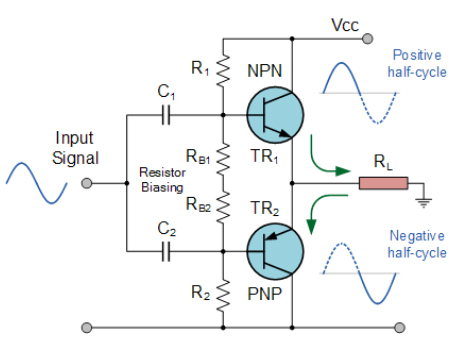
\includegraphics[scale=.8]{imagenes/amplificadorB.JPG} 
\end{center}
\begin{flushleft}
\subsection{Tipos de motor de corriente continúa}
Motor shunt: Es un motor cuyo bobinado inductor se conecta en derivación con el circuito formado por bobinas inducidas o auxiliares.

Motor compound: Su funcionamiento se origina por dos inductores independientes; uno se deriva por el circuito inducido y el otro  por la derivación con el circuito formado por el inducido; es un inductor auxiliar. Este motor tiene un rango de debilitamiento que puede ser el resultado de exceder a máxima velocidad segura del motor sin carga.
\linebreak
\linebreak
\newpage
\end{flushleft}
\begin{flushleft}
\section {Cambio de sentido de un motor de corriente continua}
Se trata de hacer girar un motor de corriente continua en los dos sentidos posibles de giro (derecha o izquierda). Primero veremos los esquemas y luego la construcción de un sencillo conmutador con madera y una punta que nos permitirá hacer el cambio de giro del motor de una forma barata, práctica y sencilla.

 Un motor cambia de sentido de giro cuando cambia la polaridad en su bornes (contactos) así de Sencillo!. Fíjate en la figura:
\end{flushleft}
\begin{center}
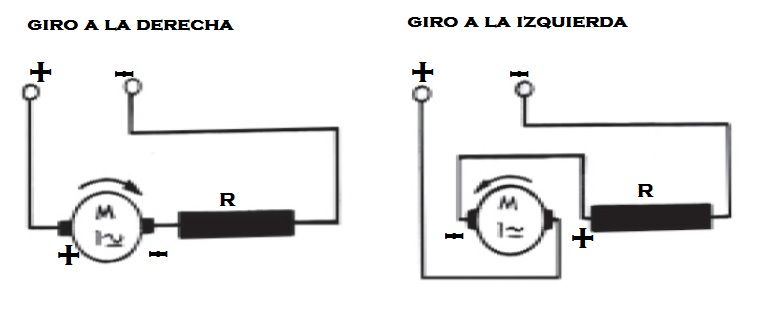
\includegraphics[scale=.5]{imagenes/1ETAPA.JPG} \linebreak
\end{center}
\begin{flushleft}
\begin{flushleft}
De esta forma tendríamos que cambiar la instalación para que girara en un sentido o en otro. Esto no es nada práctico. Lo que queremos conseguir es un esquema con el que podamos cambiar el sentido de giro mediante interruptores o mediante un simple conmutador, y sin cambiar la instalación. Aquí tienes dos esquemas:
\begin{center}
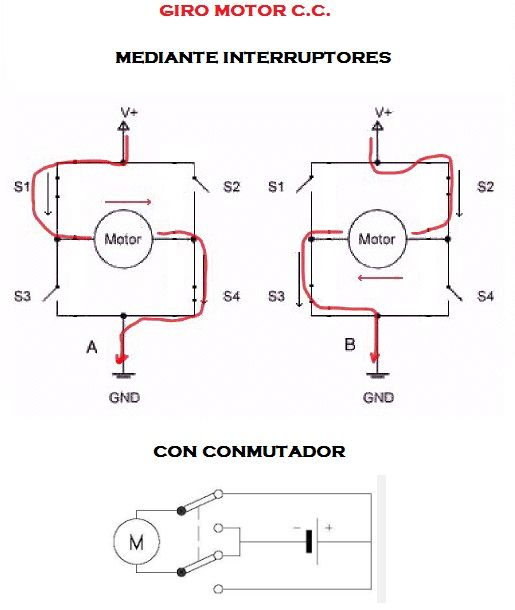
\includegraphics[scale=.5]{imagenes/sw.JPG}
\end{center}
\end{flushleft}{}

\section{Referencias bibliográficas}
\begin{flushleft}
Javier s. (2013). Cambio de sentido de un motor de corriente continua. 15/10/19, de Area Tecnologia Sitio web: https://www.areatecnologia.com/CAMBIO20DE20SENTIDO20MOTOR.html \linebreak


Eduardo R. (2019). Motor de corriente continúa; tipos y partes. 15/10/19, de tercesa Sitio web: https://tercesa.com/noticias/motor-de-corriente-continua-tipos-y-partes/\linebreak

Anonimo. (2012). Motor CC. 09/10/19, de Ecured Sitio web: https://www.ecured.cu/MotorCC

\end{flushleft}
\end{flushleft}
\end{document}

\section{se}